\chapter{Astronomy}

\section*{LEARNING OUTCOMES}
{
\begin{center}
\fcolorbox{black}{shadecolor}{%

    \parbox{0.95\textwidth}
    {%
        \small
        {
        \begin{itemize}[leftmargin=*]\itemsep0em
            \item What is space? What is present in space? How big is it?
            \item What are planets? How are they different from satellites?
            \item Discuss Earth's shape.
            \item Discuss Earth's rotation. How are day and night are caused due to the rotation of Earth?
            \item Discuss Earth's revolution around the Sun. How do seasons change due to the revolution of Earth?
            \item Differentiate between rotation and revolution.
            \end{itemize}
        }
    }%
}
\end{center}
}
\section*{DEMONSTRATIONS}
\section*{Formation of Day and Night due to Earth's Rotation}

To make the demonstration, you will need the following components:
\begin{table}[H]
    \centering
    \begin{tabular}{|c|l|c|}\hline
     \textbf{\#} & \textbf{Components} &  \textbf{Amount}\\\hline
     1 & LDR         &  1\\\hline
     2 & 10 k$\Omega$ resistor                  & 1\\\hline
     3 & Torch (or any other source of light)   &  1\\\hline
     4 & Globe                                  &  1\\\hline
     5 & Arduino UNO                            &  1\\\hline
     6 & Connecting wires                       & - \\\hline
    \end{tabular}
\end{table}
% Hardware Implementation

\subsection*{Connections}
To connect the components:
\begin{enumerate}\itemsep0em
    \item Connect the LDR and the resistor in series. Connect their junction to pin A0.
    \item Mount the Arduino board on the globe.
    \item Connect the free terminal of the LDR to 5V pin of Arduino.
    \item Connect the free terminal of the resistor to GND pin of Arduino.
\end{enumerate}
	\begin{figure}[H]
	\centering 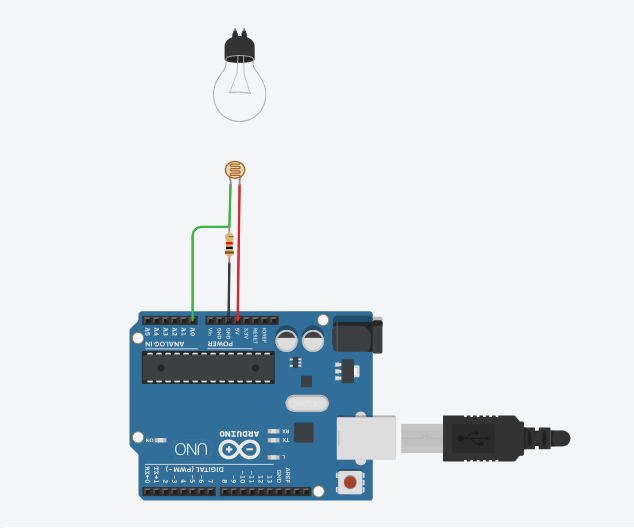
\includegraphics[scale=0.5]{astronomy.png}
	\caption{Circuit diagram of the connections}
	\end{figure}

\subsection*{Procedure}
\begin{enumerate}
    \item Connect the Arduino microcontroller to the laptop. 
    \item Open Arduino IDE and copy lst. \ref{list:day-n-night} to it. Upload your code to the Arduino board.
    \item Once the code is uploaded, open the Serial Plotter. Data should start plotting as a straight line. If the line is not straight, try to reduce the light entering the room.
    \item Turn the torch on and face it towards the LDR. 
    \item While holding the torch at its place, start rotating the globe. The plot should start to slope down indicating a decrease in the light falling on the LDR.
\end{enumerate}
\begin{lstlisting}[language=Arduino, numbers=none, caption={Arduino code for reading the variation in LDR resistance}, captionpos=b, label={list:day-n-night}, breaklines=true]
int ldr=A0;  

void setup() 
{
  // put your setup code here, to run once:
  pinMode(ldr, INPUT);    
  // A0 is declared an input peripheral
  Serial.begin(9600);
}

void loop() 
{
  // put your main code here, to run repeatedly:
  int intensity = analogRead(ldr);  
  // The intensity of light on the LDR is recorded
  Serial.println(intensity);        
  // The light intensity is printed either 
  // on Serial Monitor or on Serial Plotter
}
\end{lstlisting}
\subsection*{Precautions}
\begin{itemize}[leftmargin=*]
\item For this experiment, try to keep the lighting in the room to a minimum. Although LDR is not very sensitive, stray light beams may affect the results of this experiment.
\end{itemize}

\subsection*{Additional Notes}
\begin{itemize}[leftmargin=*]
\item If a globe is not available, use a hollow ball and pass a straw through it by drilling holes on it. If the size of the ball is small, Arduino board may not be mounted on the ball and can be placed separately.  
\item The concept of \textbf{time zones} can be communicated by mounting two or more LDRs on the globe and displaying their results simultaneously.
 \end{itemize}

\begin{figure}[!ht]
\centering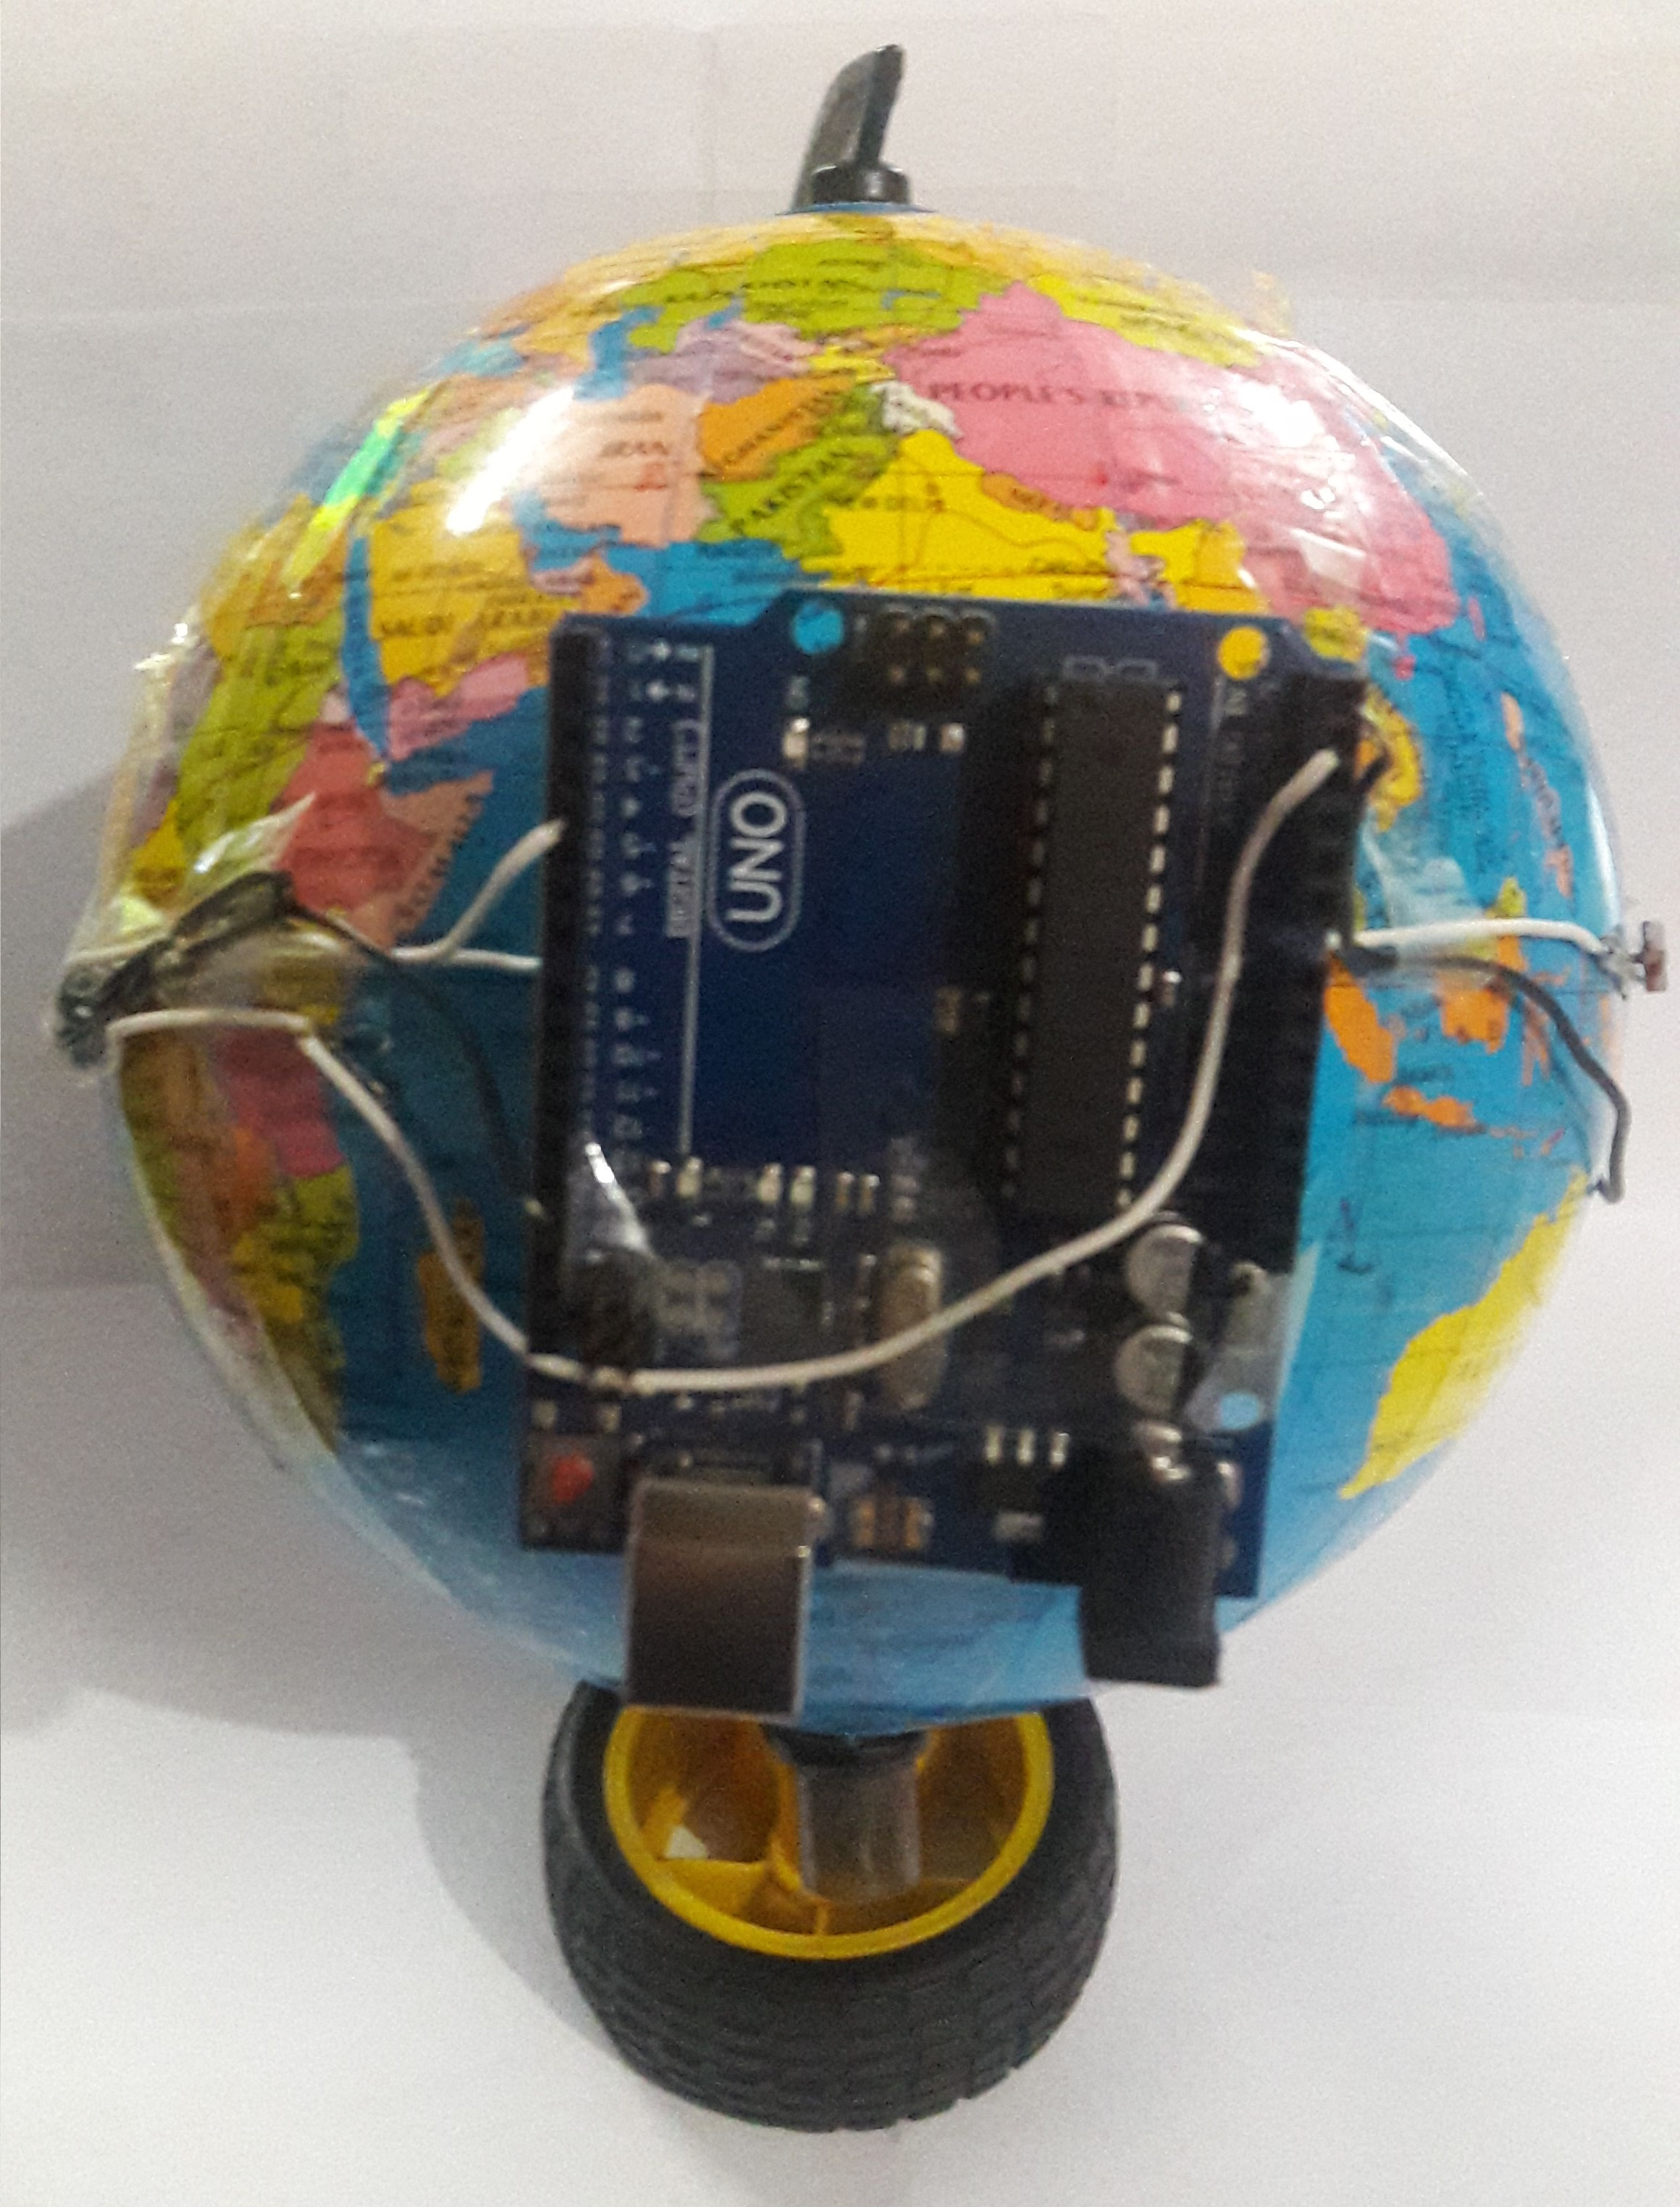
\includegraphics[scale=0.08]{astronomy-hardware-1.jpeg}
\caption{Hardware of the demonstration}
\end{figure}